\subsection{Sơ đồ tuần tự} \label{sec:sequence_diagram}

Trong khi sơ đồ hoạt động tập trung vào luồng xử lý logic và các điểm quyết định, sơ đồ tuần tự đóng vai trò chi tiết hóa sự tương tác giữa các đối tượng trong hệ thống theo trình tự thời gian. Các sơ đồ này làm rõ cách thức các dịch vụ Backend, cơ sở dữ liệu và trợ lý ảo AI phối hợp truyền tải thông điệp để hoàn thành một nghiệp vụ cụ thể. Đây là cơ sở quan trọng để nhóm xác định các phương thức và cấu trúc giao tiếp giữa các Microservices.

Các hình từ \ref{fig:seq_find_product} đến \ref{fig:seq_report} trình bày các sơ đồ hoạt động cho những trường hợp sử dụng cốt lõi của hệ thống. Các sơ đồ còn lại sẽ được biểu diễn ở phần phụ lục \ref{sec:appx_activity_diagram}.

\begin{figure}[H]
    \centering
    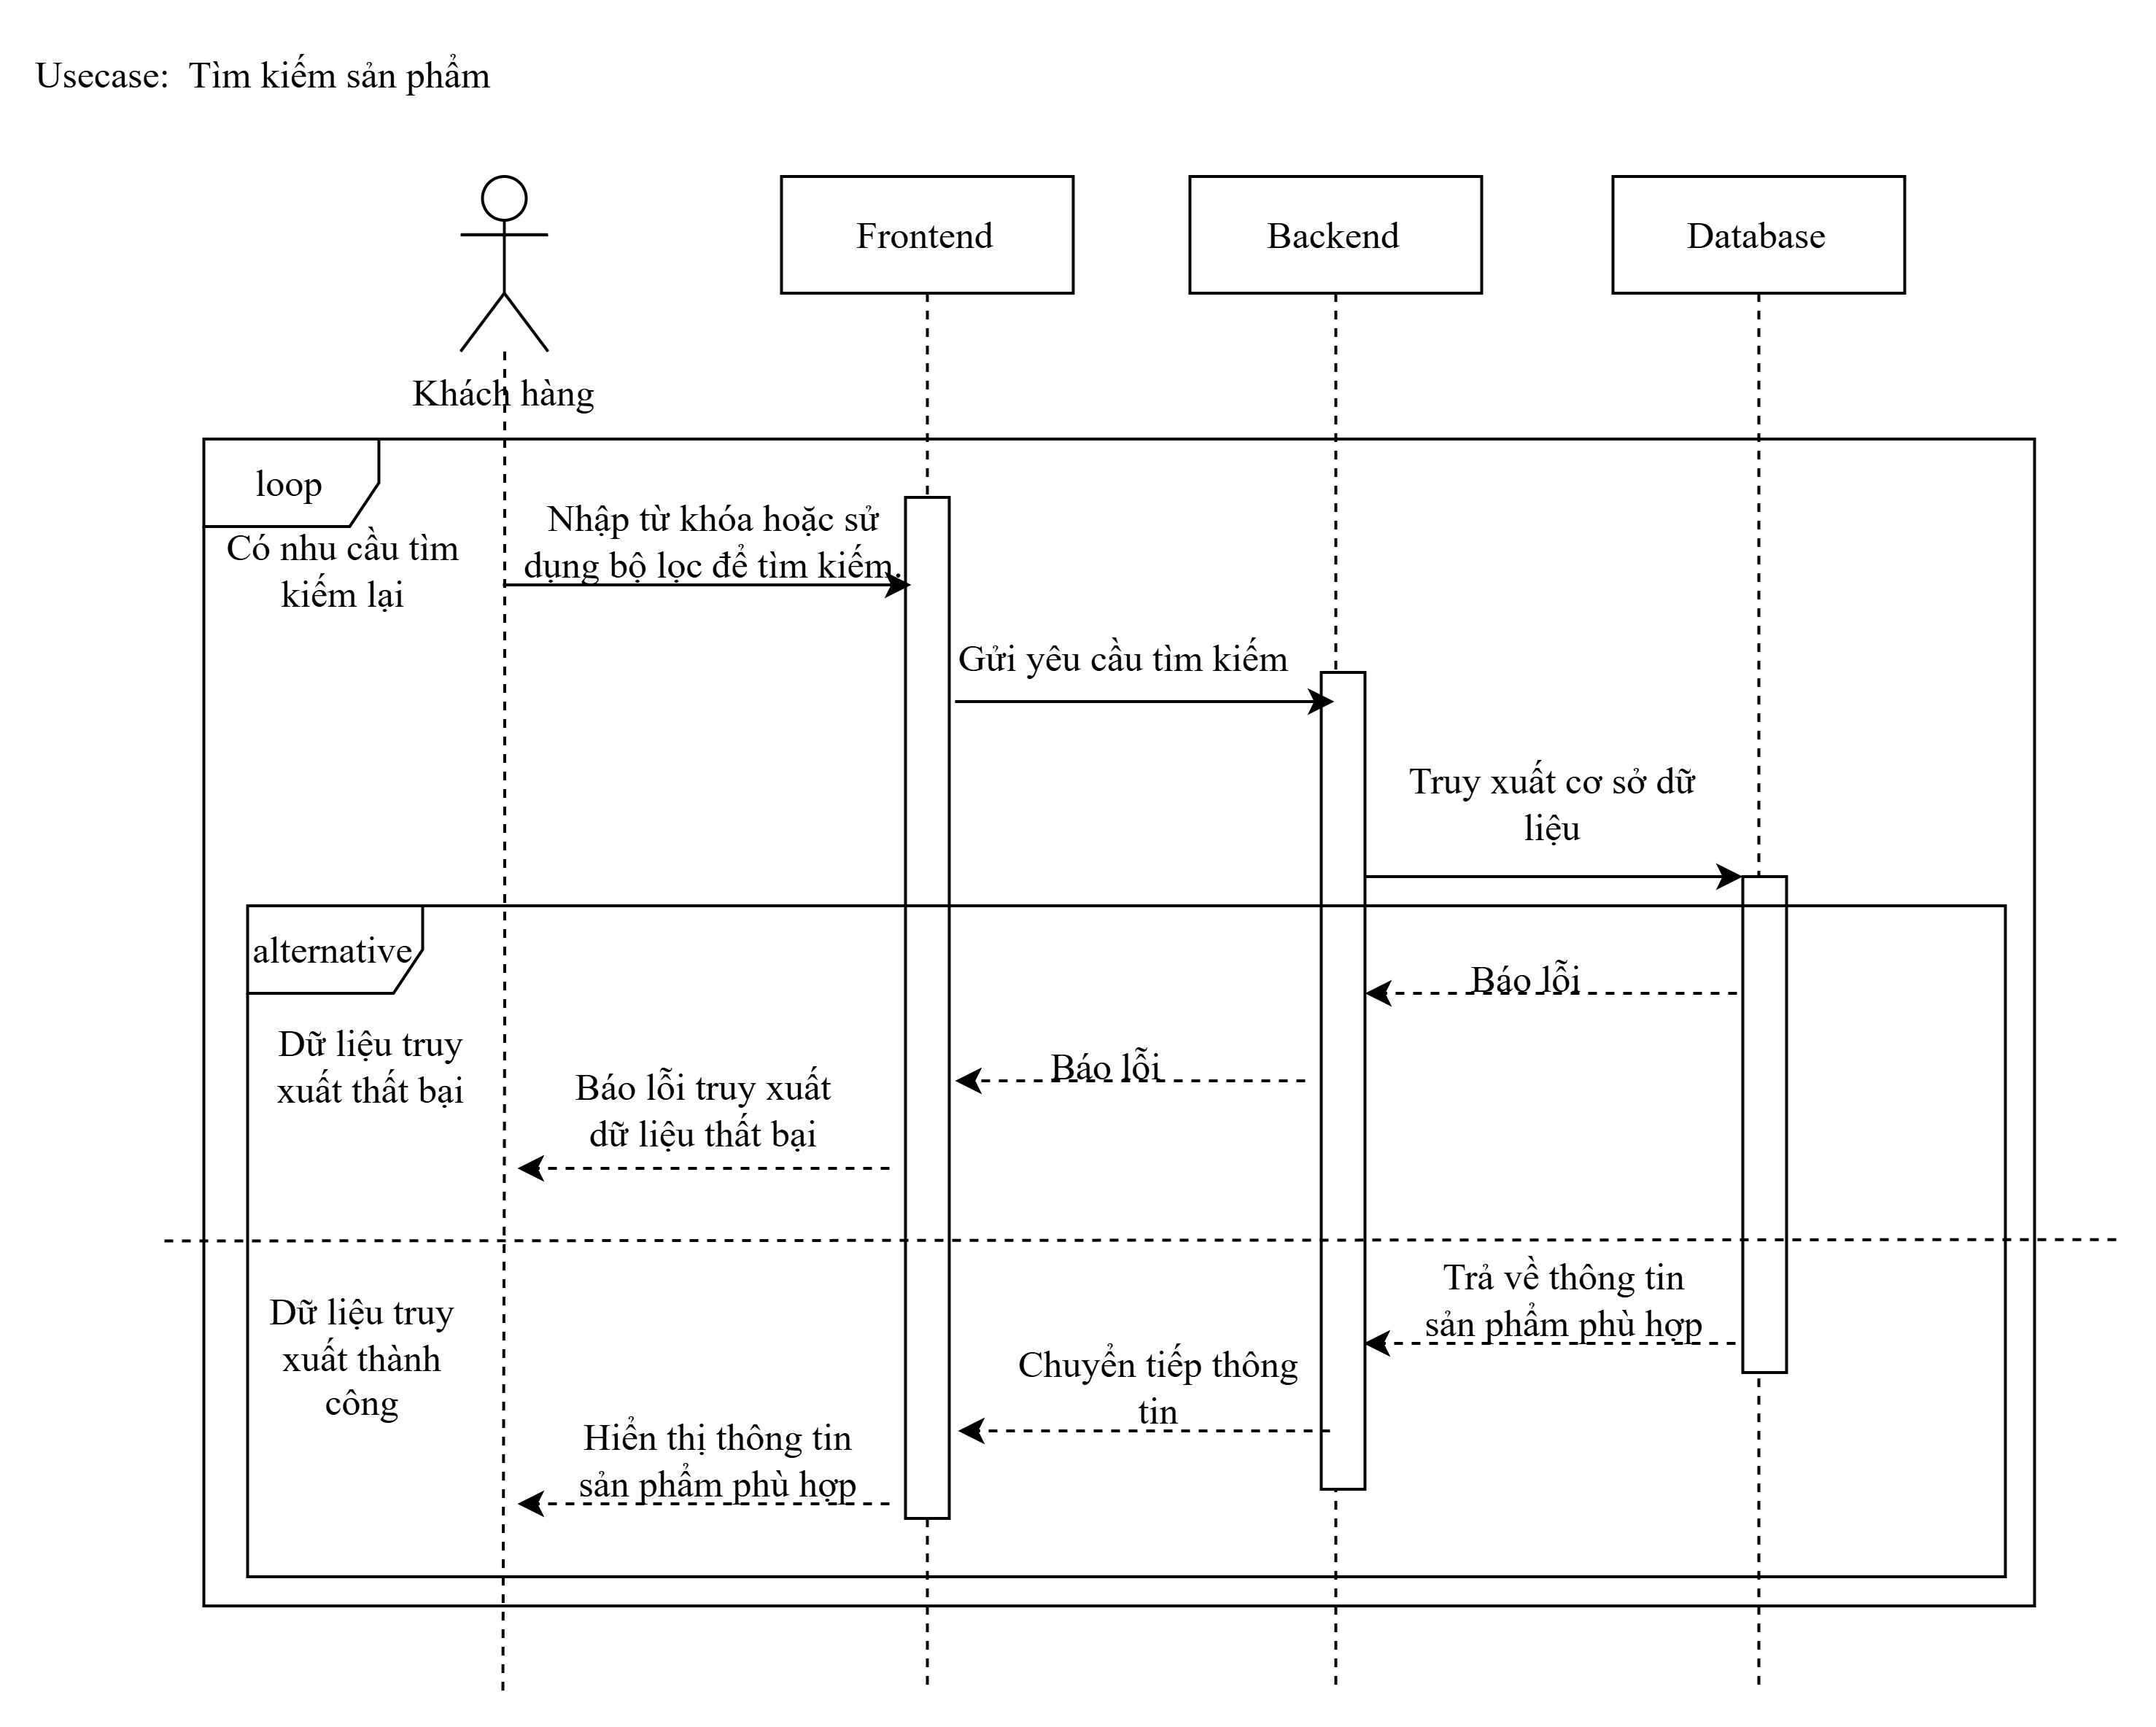
\includegraphics[width=1.0\linewidth]{images/chap3/sequence_diagram/find_product.png}
   \vspace{0.5cm} \caption{Sơ đồ tuần tự Tìm kiếm sản phẩm}
    \label{fig:seq_find_product}
\end{figure}
Hình \ref{fig:seq_find_product} mô tả luồng khi người dùng gửi từ khóa hoặc bộ lọc. Controller xử lý yêu cầu, truy vấn danh sách sản phẩm từ Database thỏa mãn điều kiện và trả về danh sách kết quả hiển thị cho người dùng.

\begin{figure}[H]
    \centering
    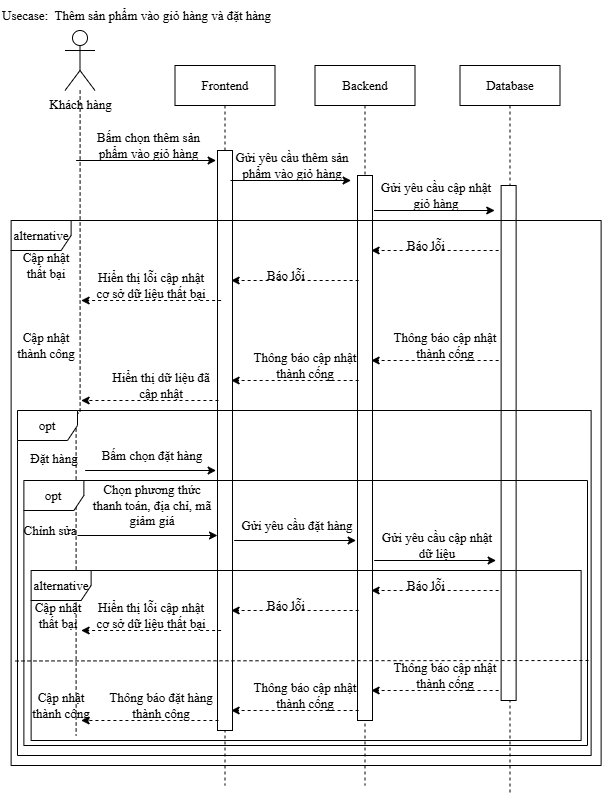
\includegraphics[width=1.0\linewidth]{images/chap3/sequence_diagram/add_to_cart_and_checkout.png}
   \vspace{0.5cm} \caption{Sơ đồ tuần tự Thêm vào giỏ và Đặt hàng}
    \label{fig:seq_cart_checkout}
\end{figure}
Hình \ref{fig:seq_cart_checkout} mô tả sơ đồ phức tạp mô tả chuỗi hành động: Kiểm tra tồn kho khi thêm vào giỏ -> Cập nhật giỏ hàng -> Khởi tạo đơn hàng (Order) -> Lưu chi tiết đơn hàng (Order Details) và xác nhận đặt hàng thành công.

\begin{figure}[H]
    \centering
    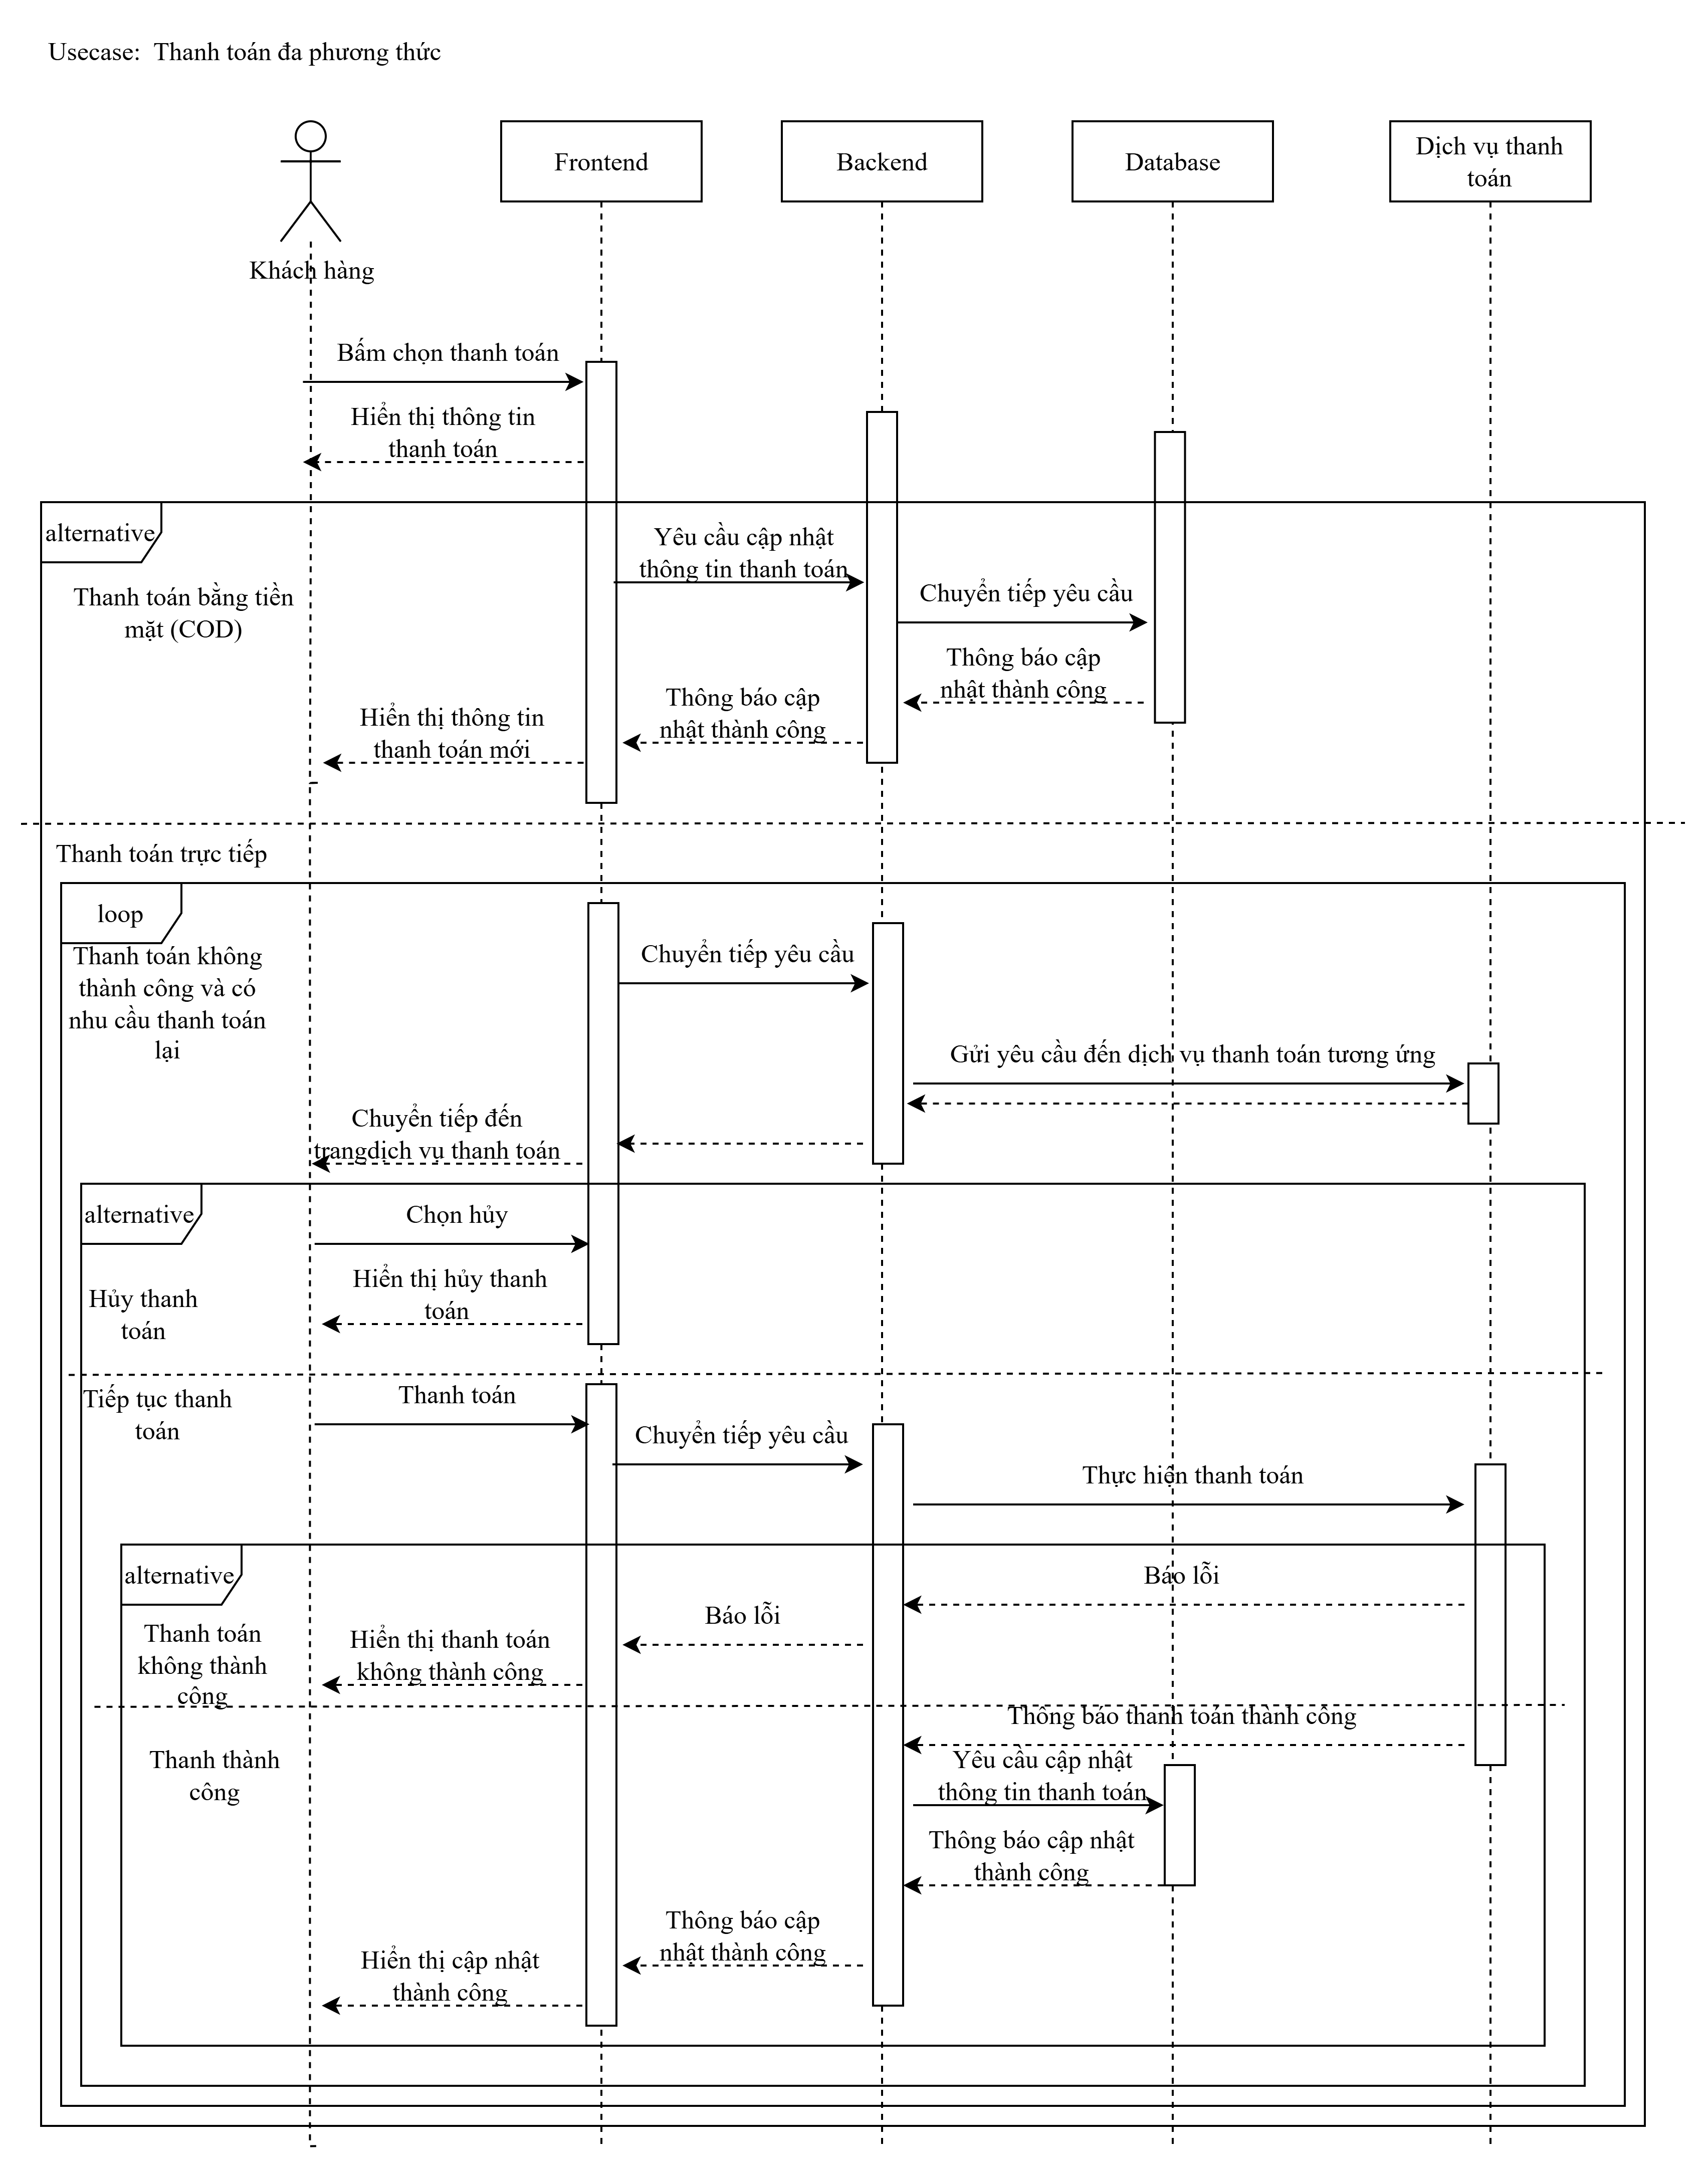
\includegraphics[width=0.9\linewidth]{images/chap3/sequence_diagram/multiple_payment_method.png}
   \vspace{0.5cm} \caption{Sơ đồ tuần tự Thanh toán đa phương thức}
    \label{fig:seq_payment}
\end{figure}
Hình \ref{fig:seq_payment} mô tả việc người dùng chọn phương thức thanh toán. Hệ thống có thể tương tác với cổng thanh toán bên ngoài (API) hoặc xử lý thanh toán nội bộ, sau đó cập nhật trạng thái thanh toán cho đơn hàng.

\begin{figure}[H]
    \centering
    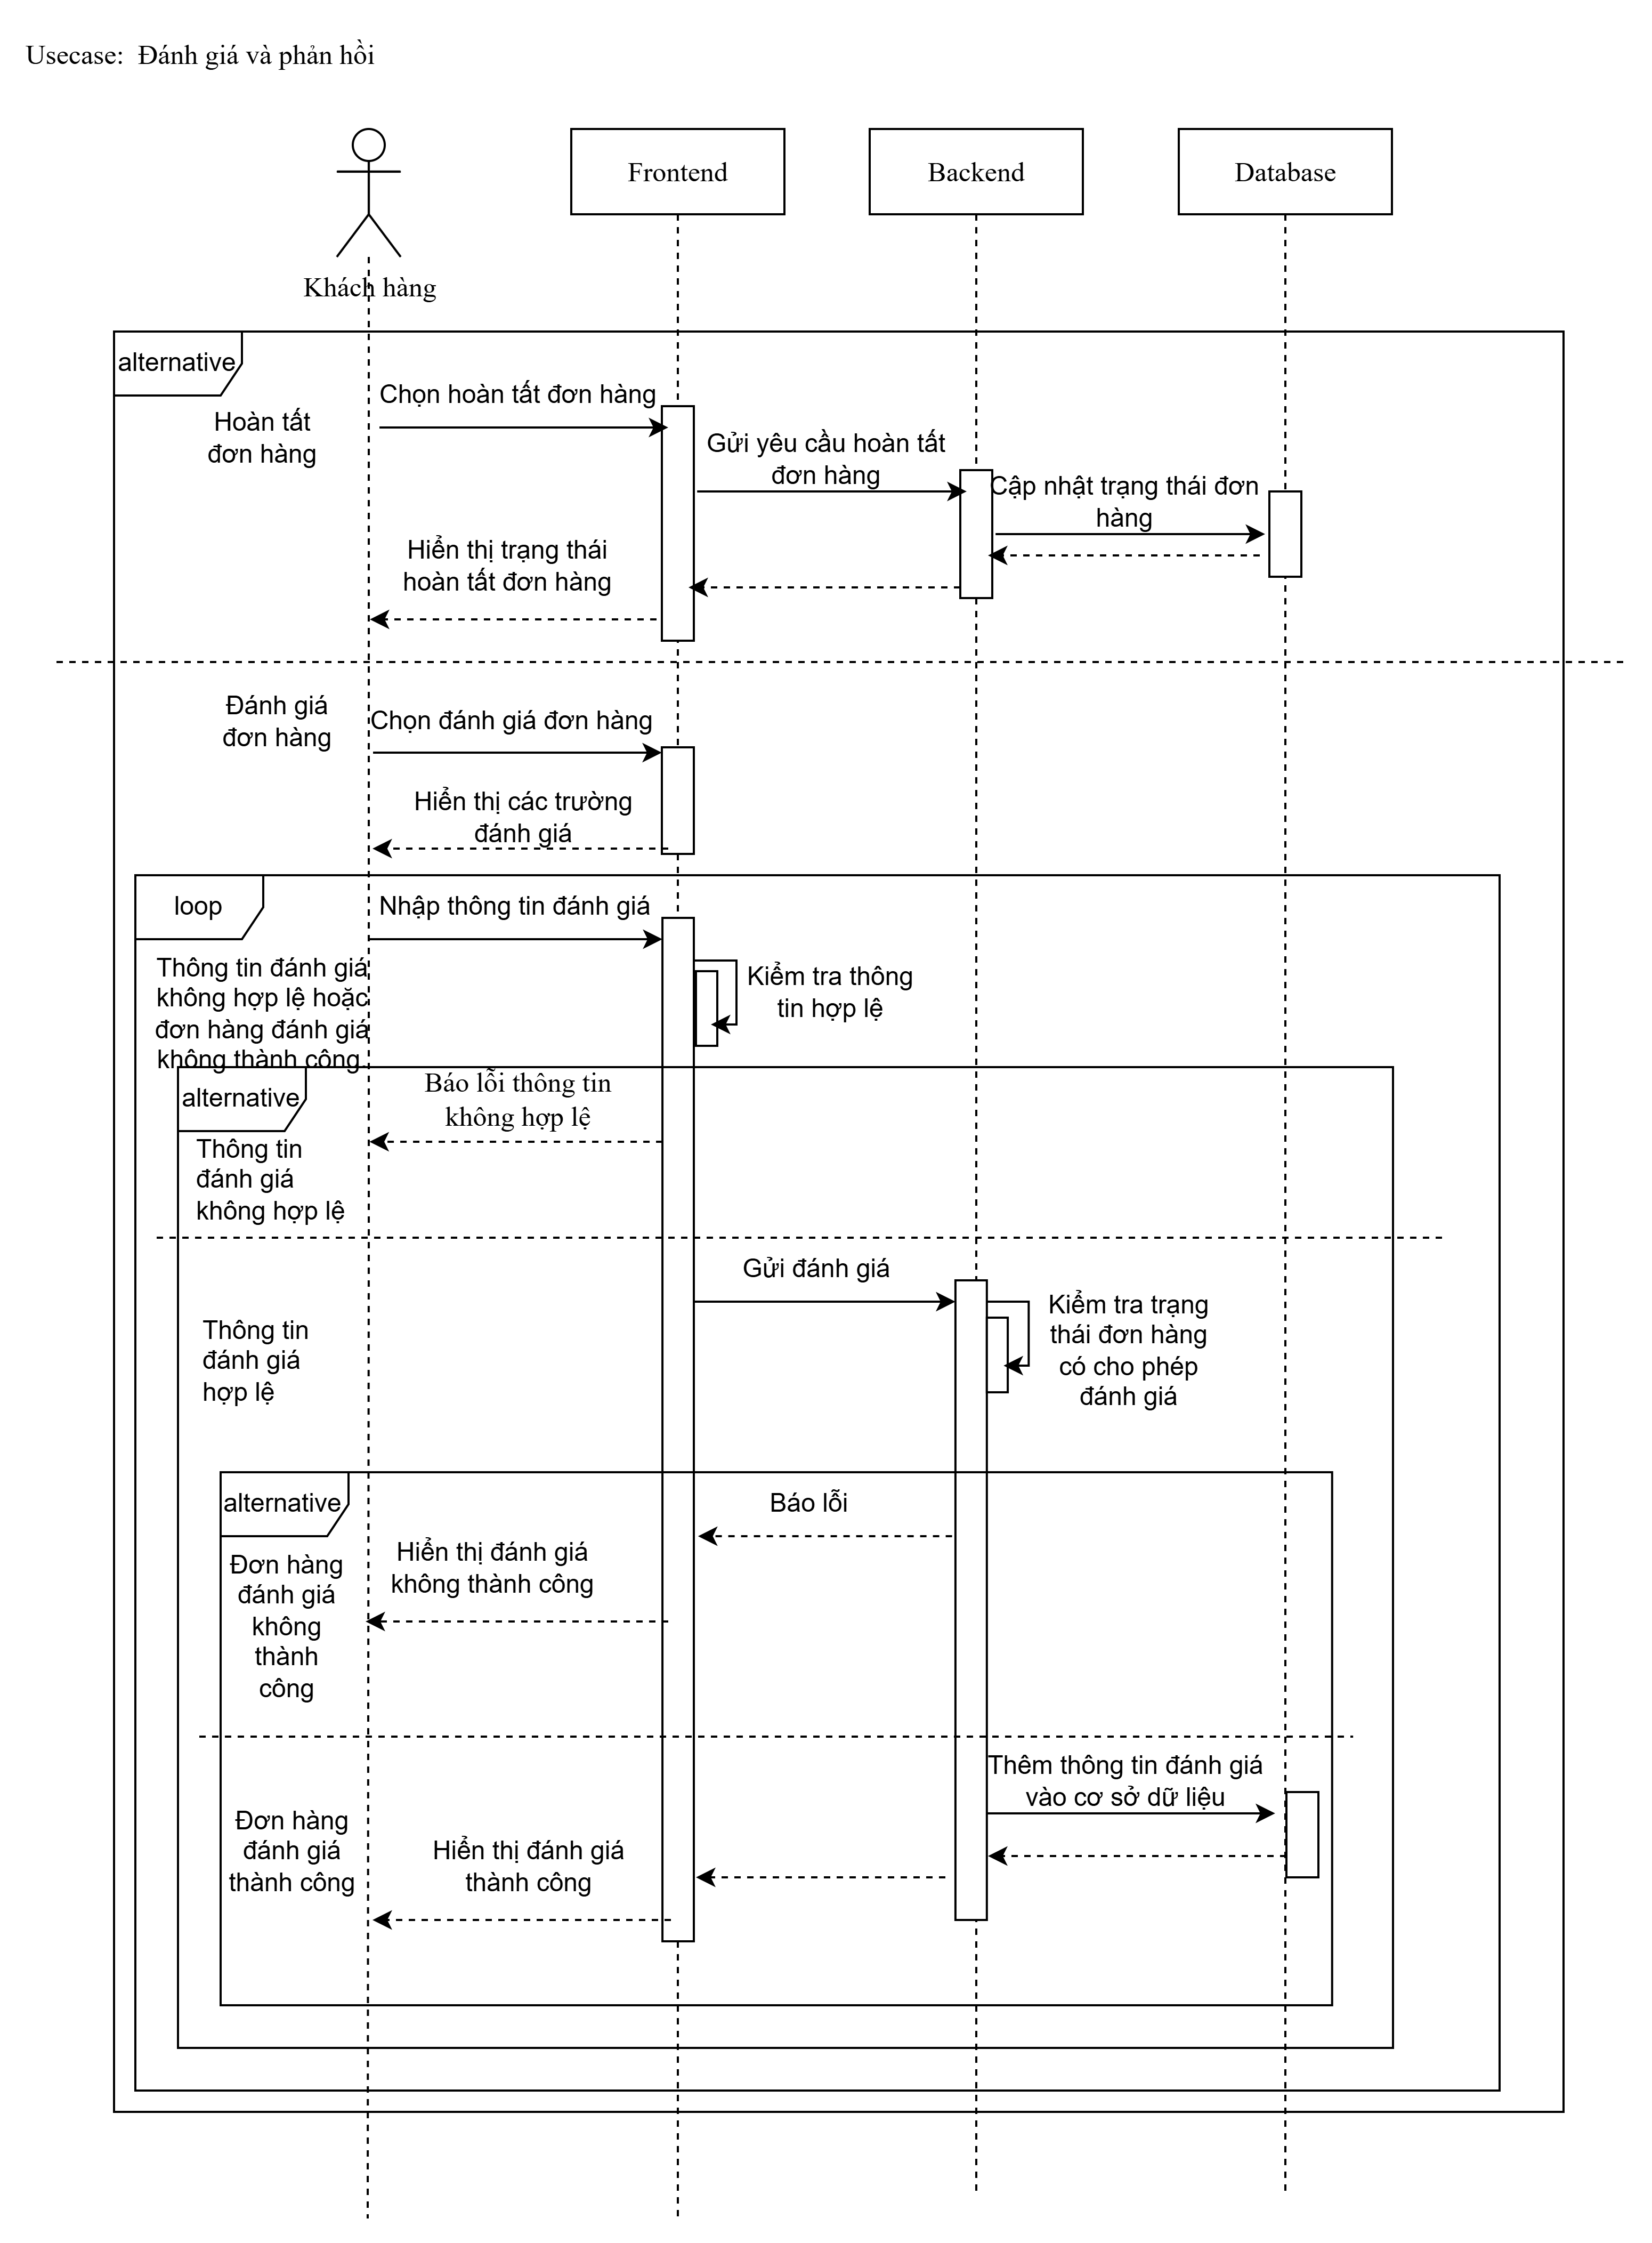
\includegraphics[width=0.9\linewidth]{images/chap3/sequence_diagram/customer_feedback.png}
   \vspace{0.5cm} \caption{Sơ đồ tuần tự Gửi phản hồi khách hàng}
    \label{fig:seq_feedback}
\end{figure}
Hình \ref{fig:seq_feedback} cho thấy sau khi hoàn tất đơn hàng, người dùng gửi đánh giá. Hệ thống lưu trữ nội dung phản hồi và liên kết nó với sản phẩm hoặc đơn hàng tương ứng trong cơ sở dữ liệu.

\begin{figure}[H]
    \centering
    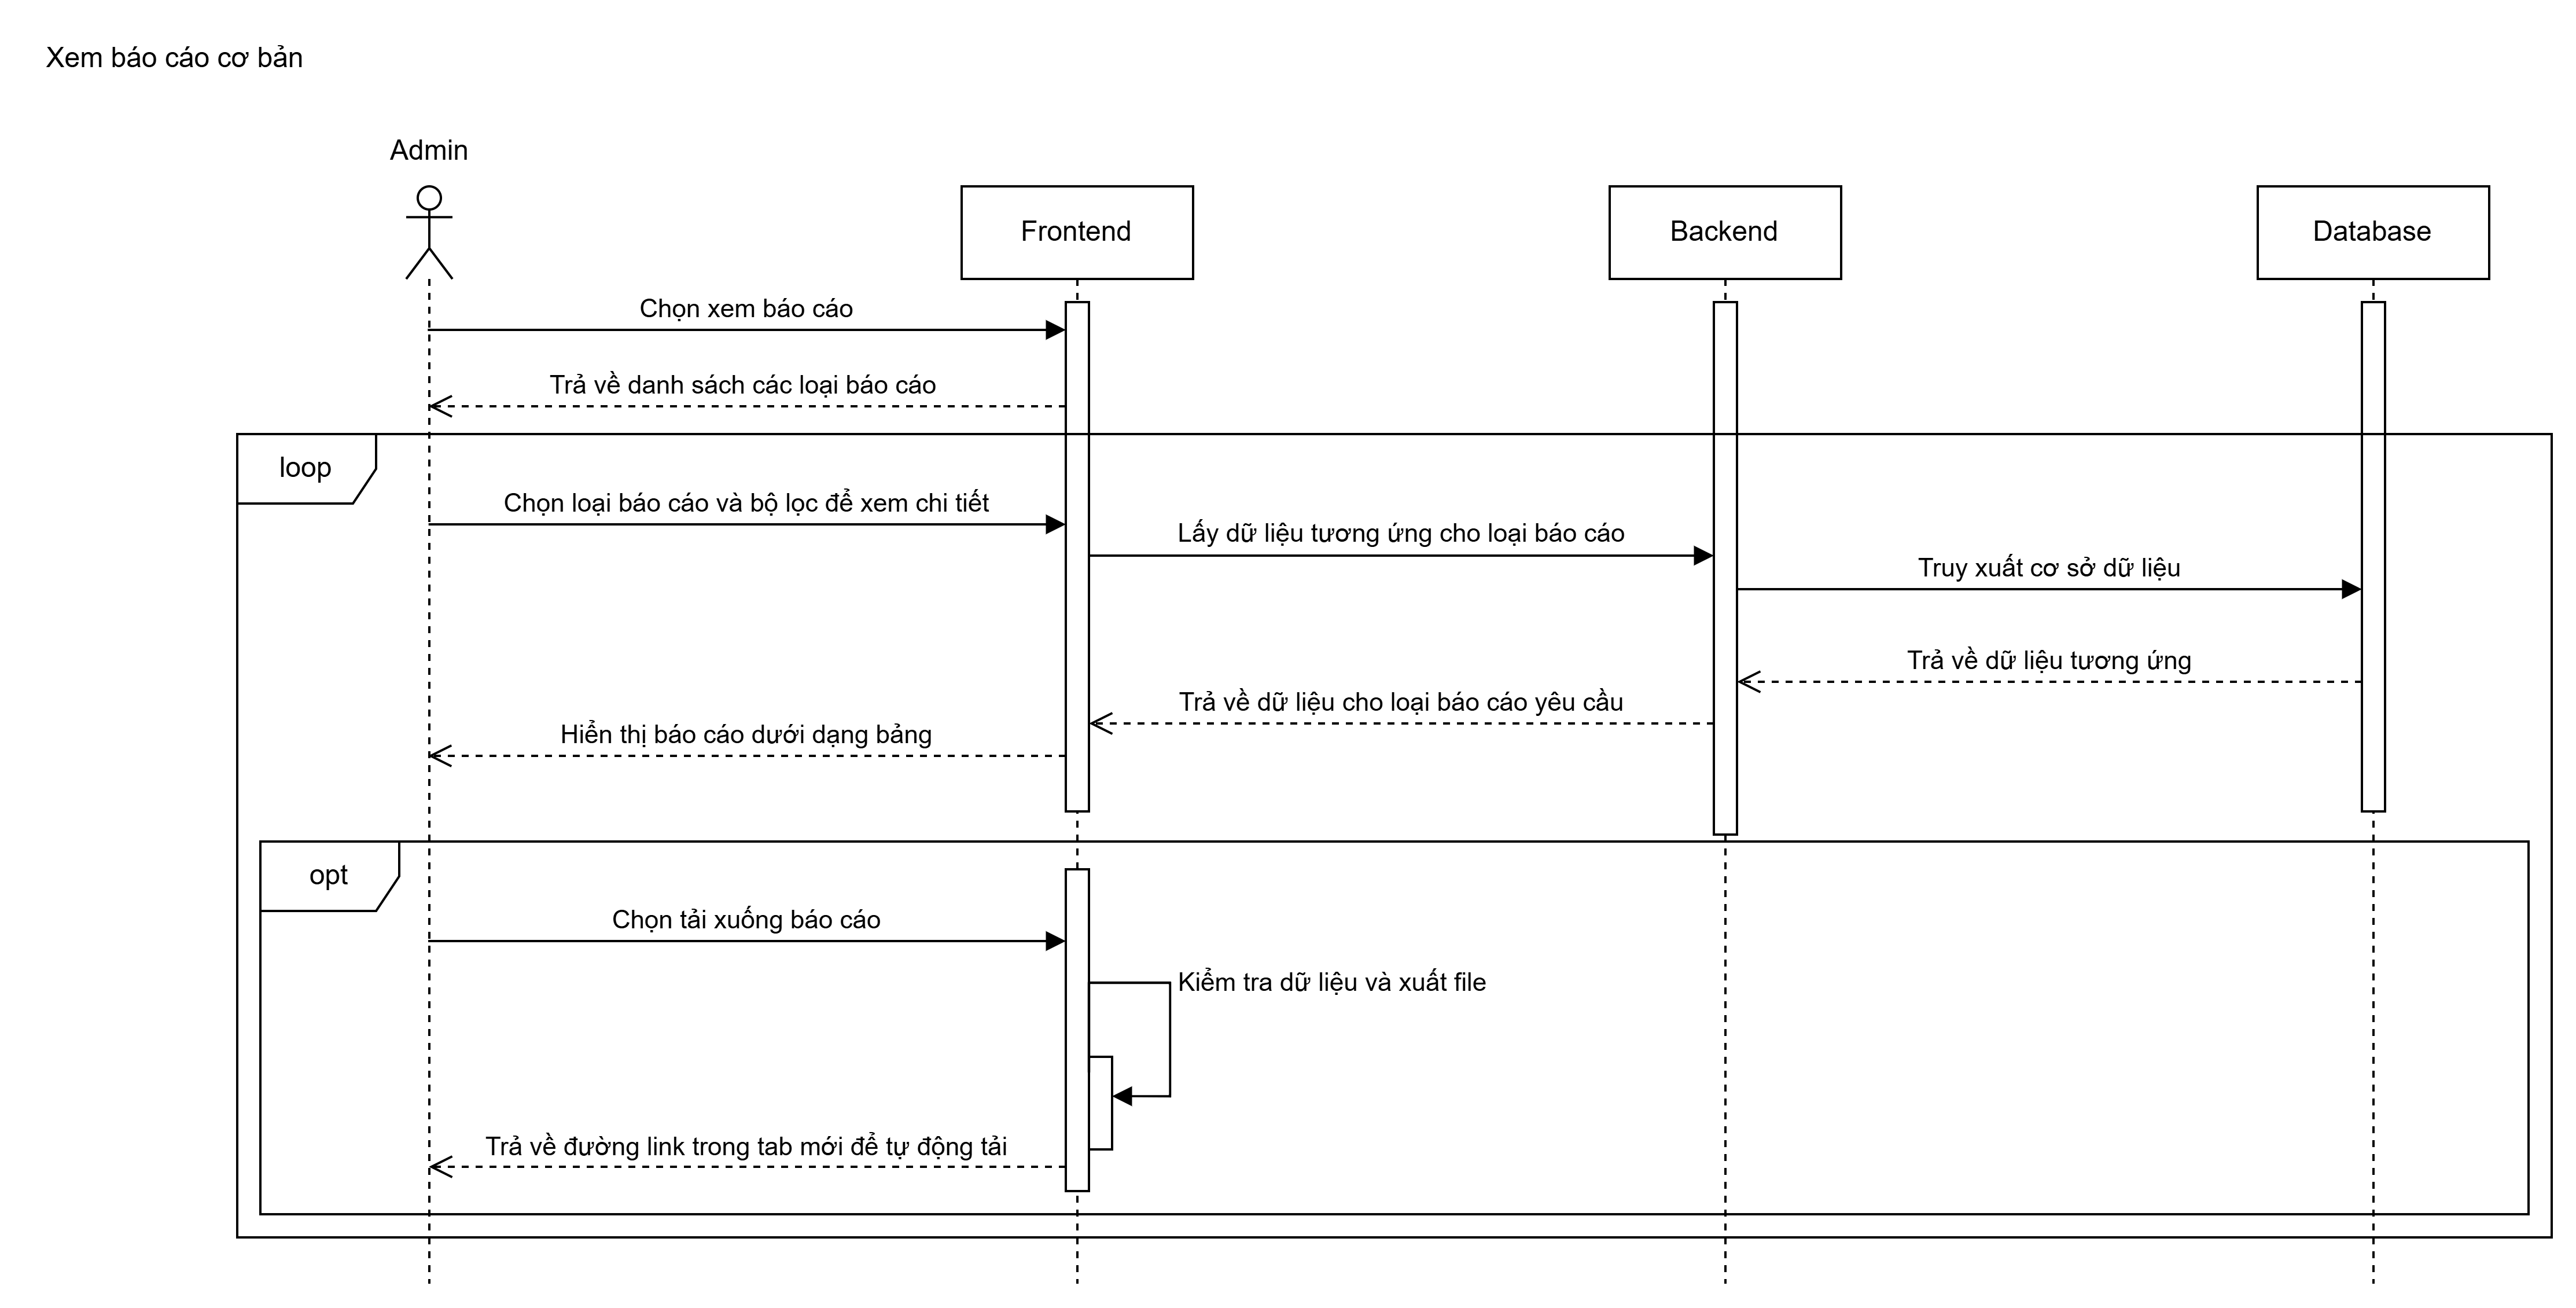
\includegraphics[width=0.9\linewidth]{images/chap3/sequence_diagram/view_basic_report.png}
   \vspace{0.5cm} \caption{Sơ đồ tuần tự Xem báo cáo thống kê}
    \label{fig:seq_report}
\end{figure}
Hình \ref{fig:seq_report} biểu diễn luồng khi admin chọn loại báo cáo và khoảng thời gian. Hệ thống tổng hợp dữ liệu từ các bảng Order, Product, Payment,... tính toán các chỉ số và hiển thị biểu đồ hoặc bảng số liệu.

\begin{figure}[H]
    \centering
    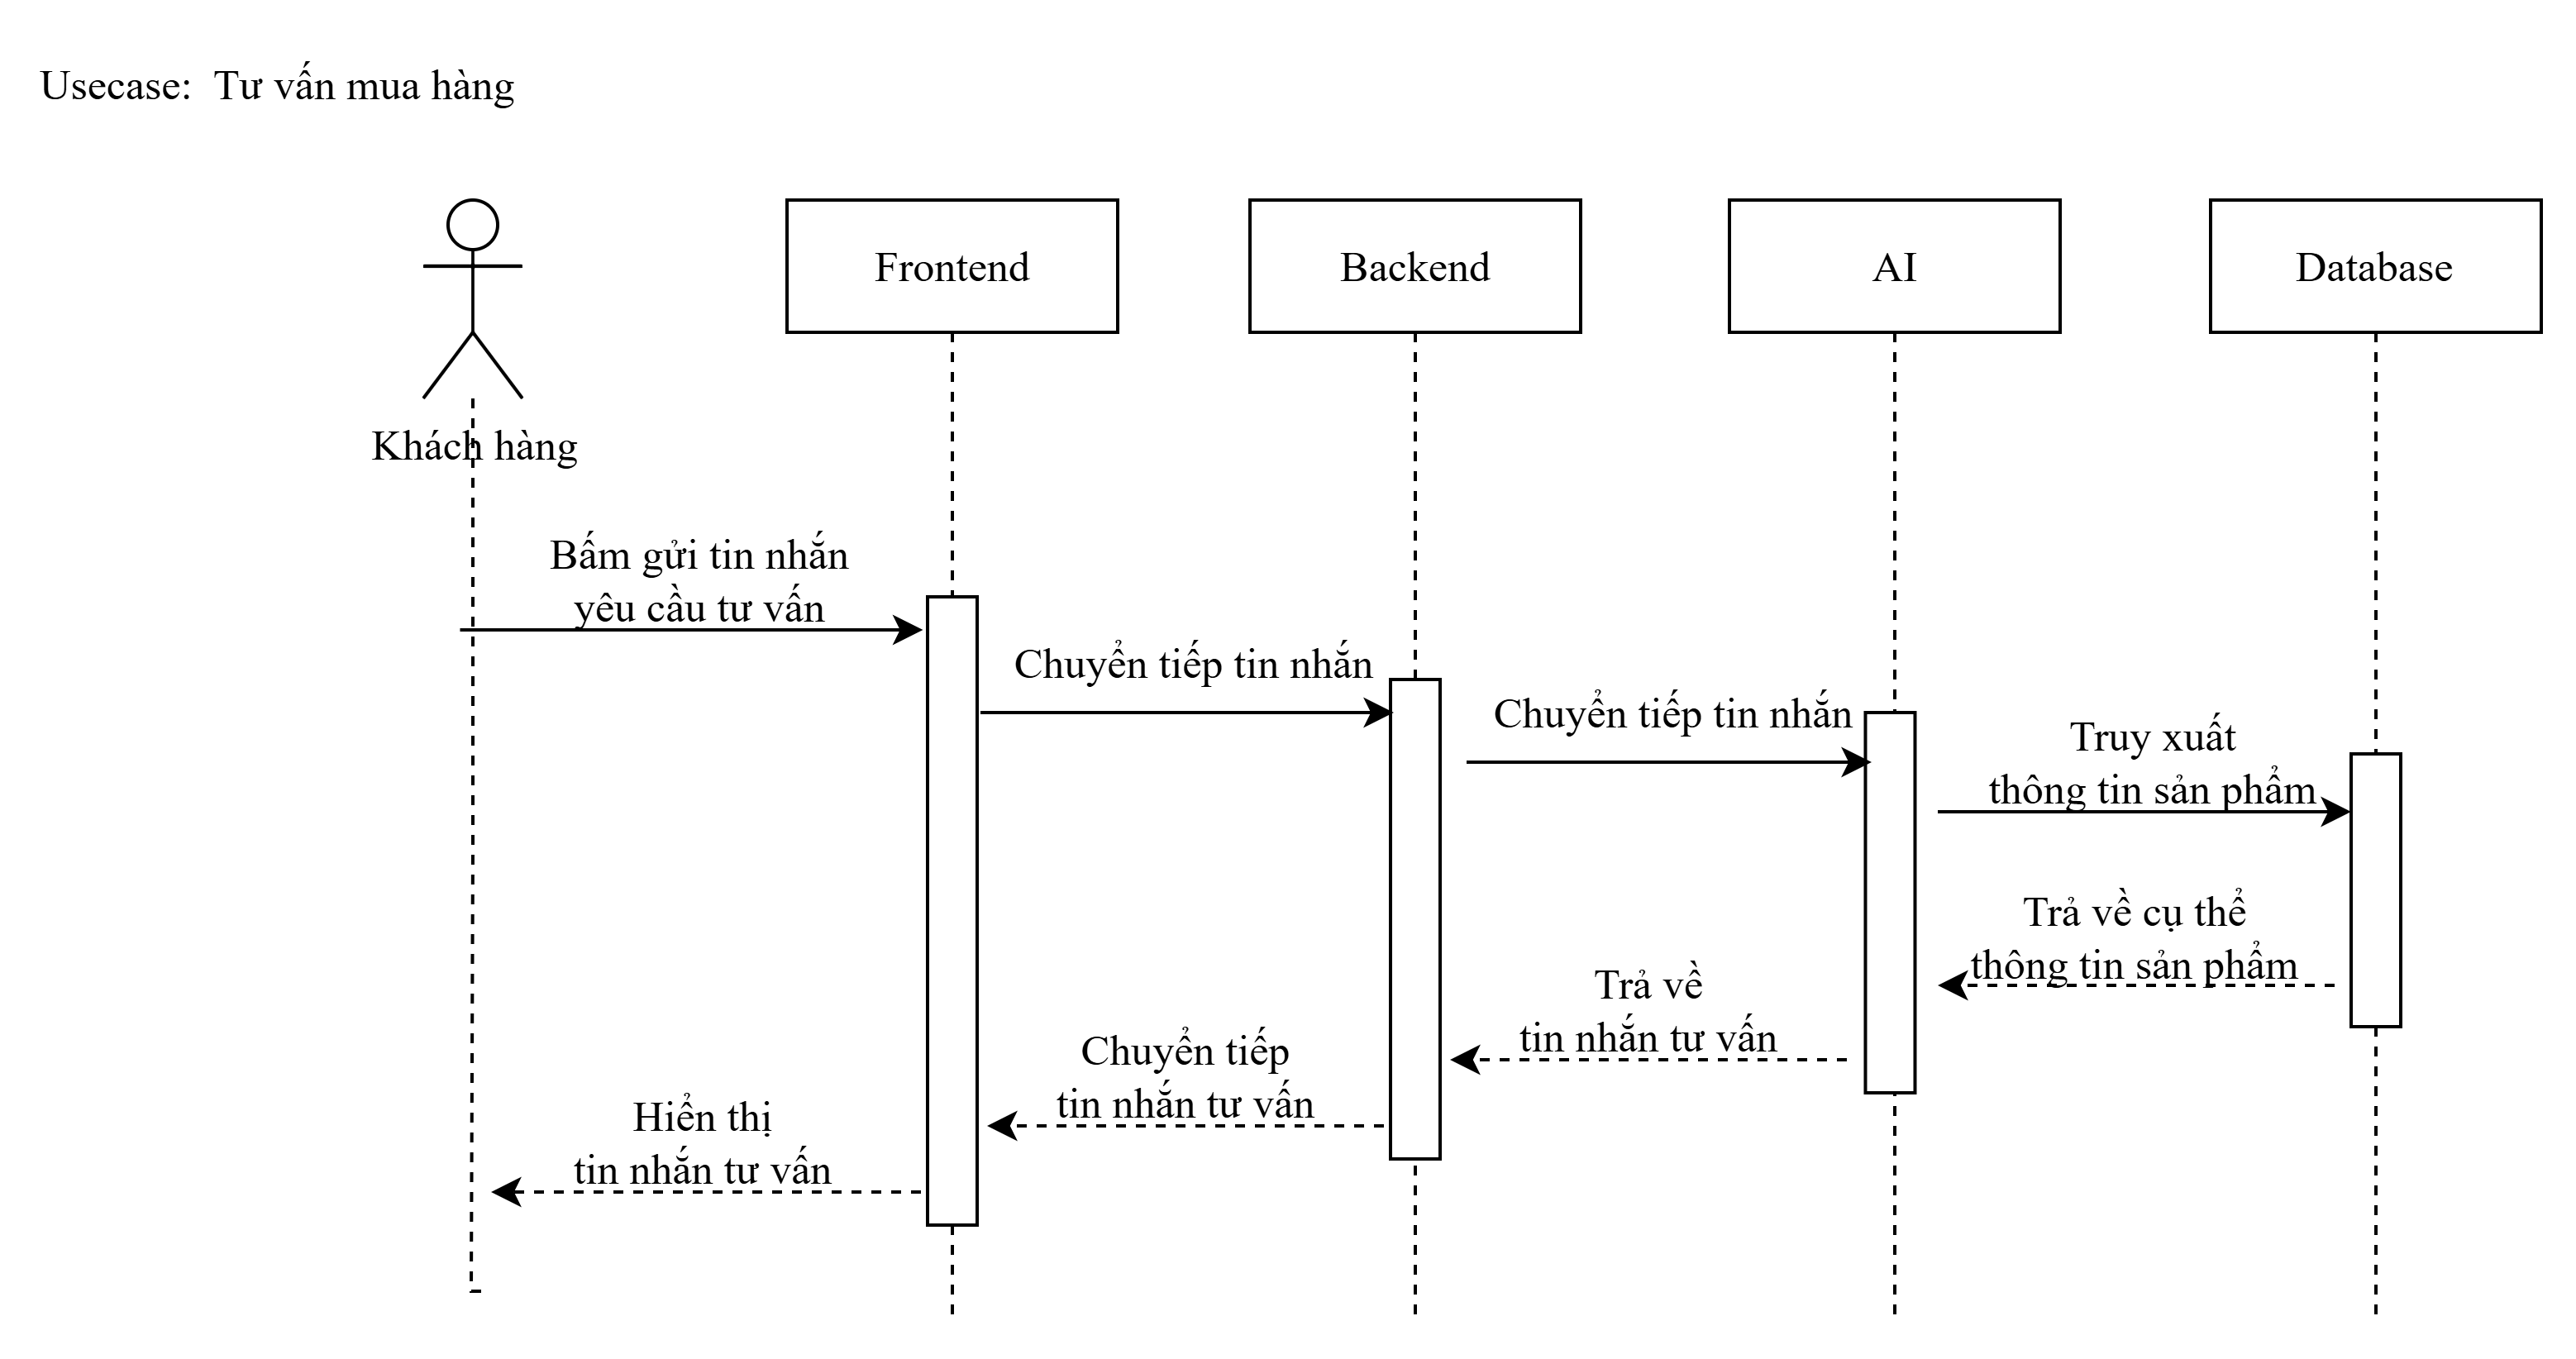
\includegraphics[width=0.9\linewidth]{images/chap3/sequence_diagram/shopping_consulting.png}
   \vspace{0.5cm} \caption{Sơ đồ tuần tự Tư vấn mua sắm}
    \label{fig:seq_consulting}
\end{figure}
Mô tả luồng tin nhắn giữa Khách hàng và Nhân viên hỗ trợ/Hệ thống Chatbot để giải đáp thắc mắc về sản phẩm trước khi mua.

\begin{figure}[H]
    \centering
    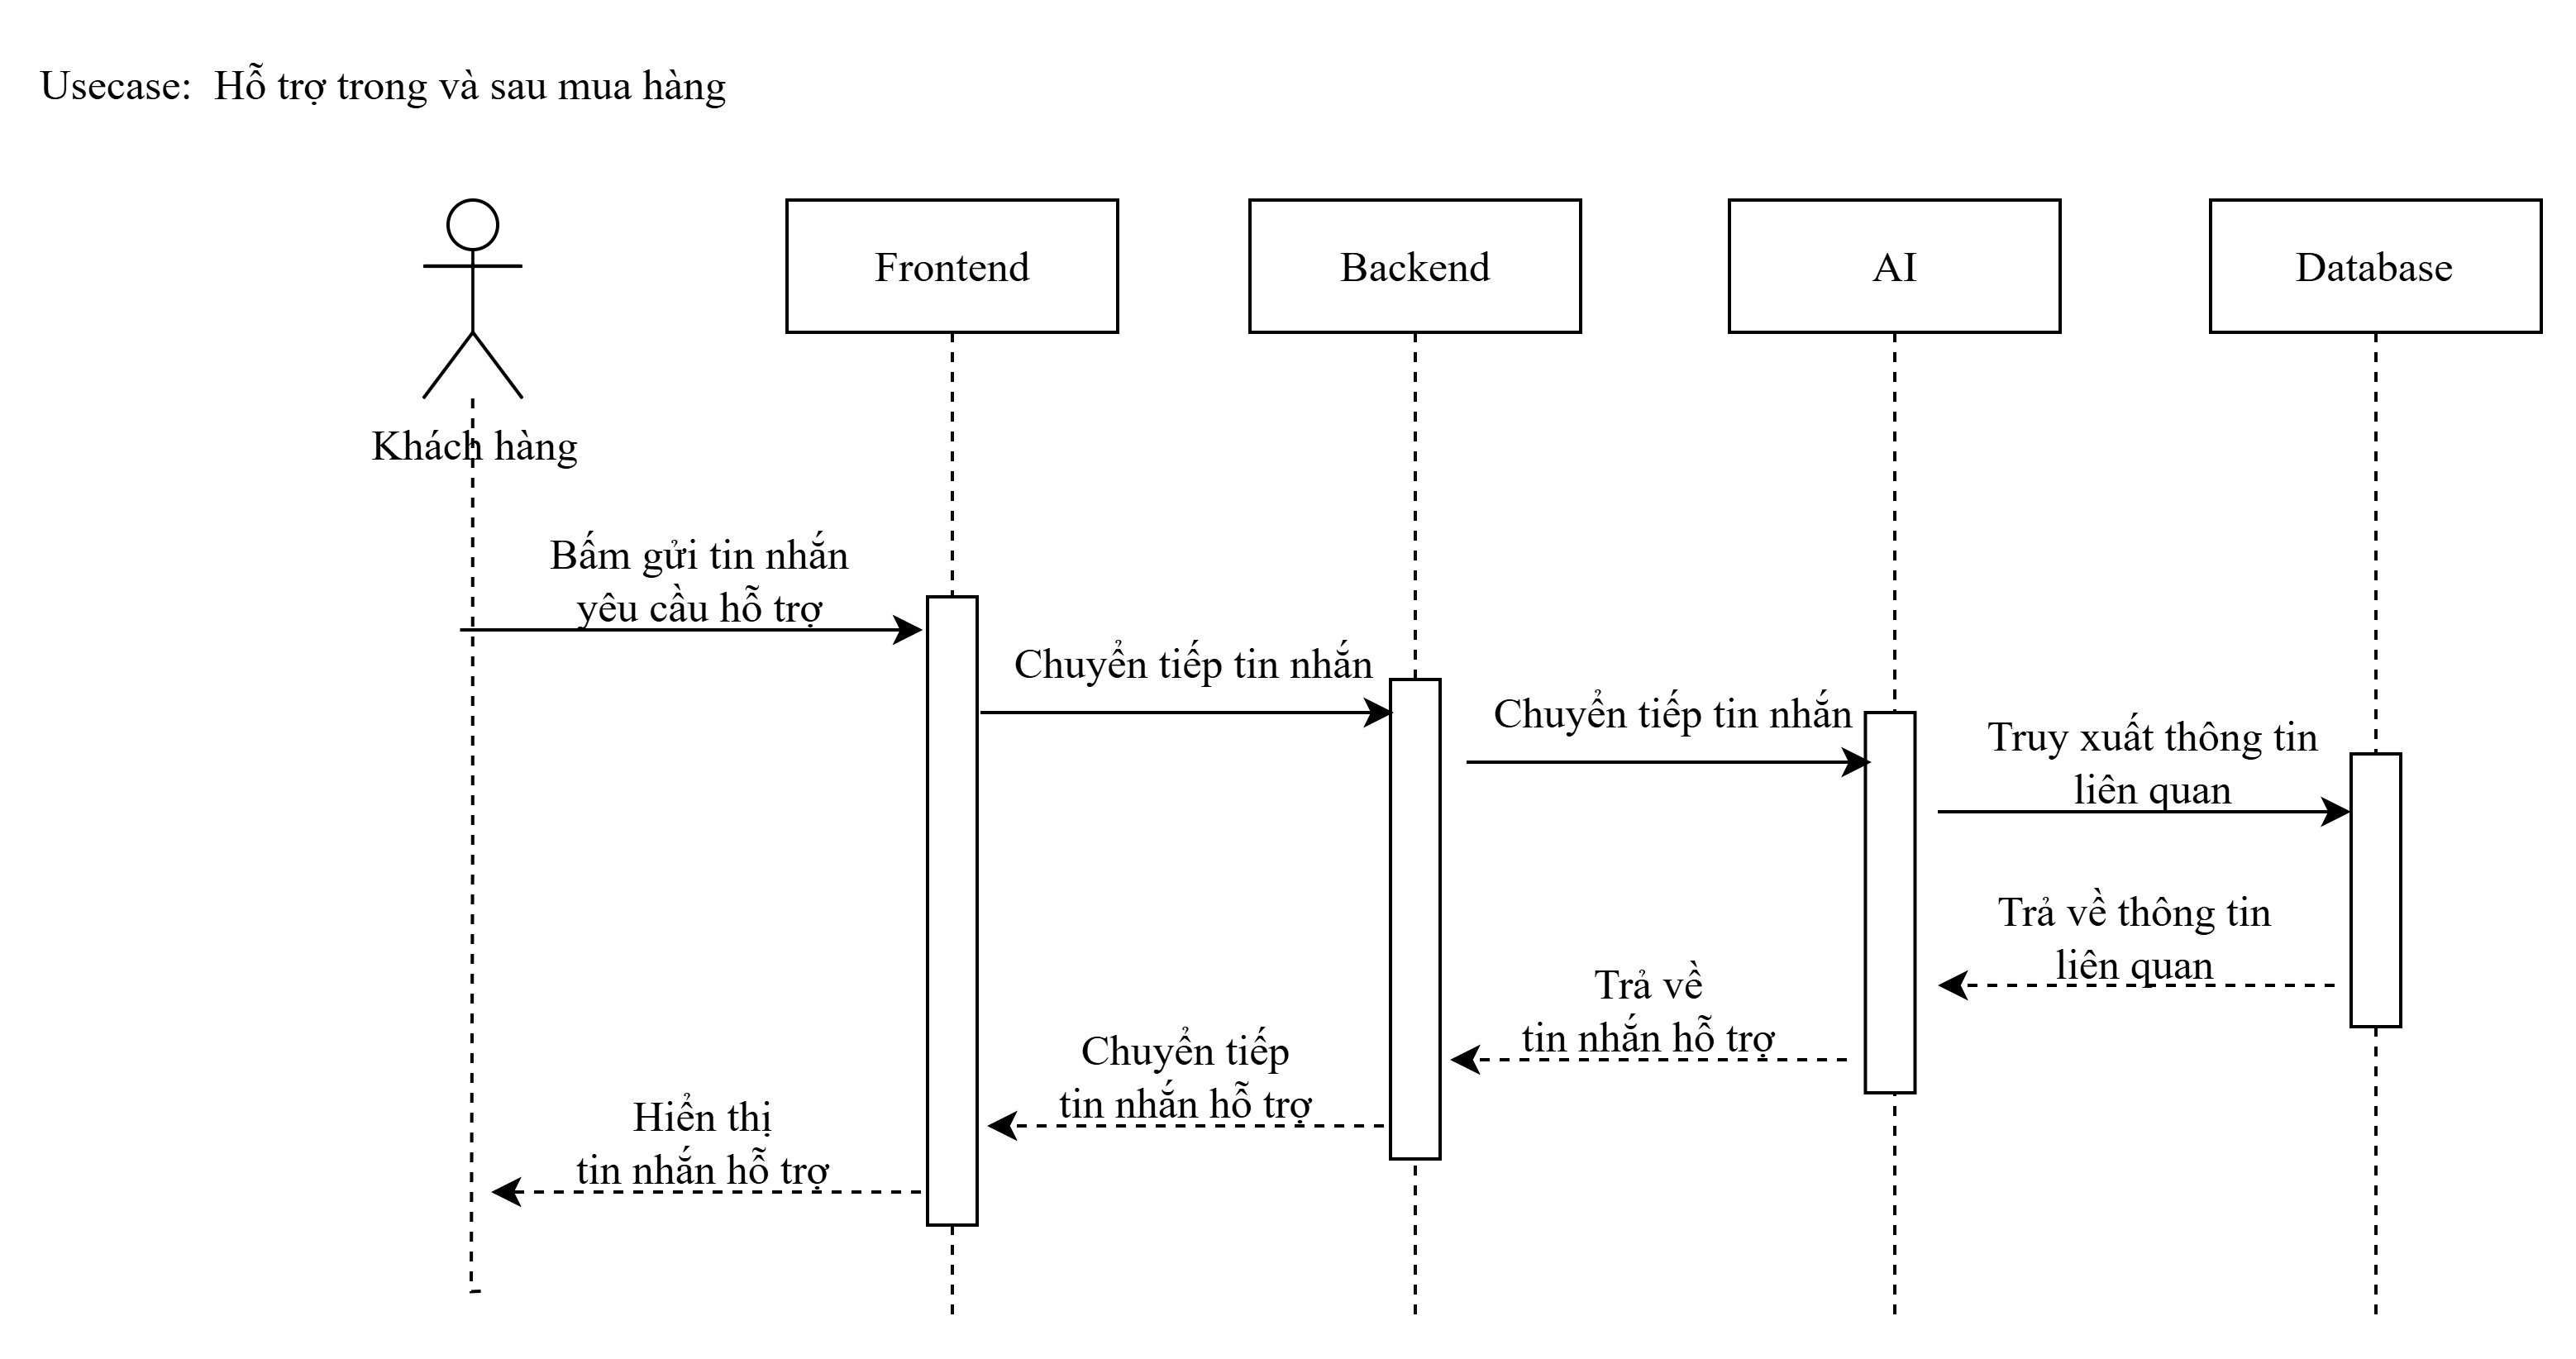
\includegraphics[width=0.9\linewidth]{images/chap3/sequence_diagram/shopping_support.png}
   \vspace{0.5cm} \caption{Sơ đồ tuần tự Hỗ trợ sau mua hàng}
    \label{fig:seq_shopping_support}
\end{figure}
Quy trình xử lý các khiếu nại hoặc yêu cầu bảo hành. Nhân viên kiểm tra thông tin đơn hàng trên hệ thống và ghi nhận kết quả xử lý hỗ trợ.
